\chapter{Resultados}
\label{sec:results}

A análise dos nossos resultados inicia-se com um resumo de alto nível do desempenho do IVF/SPEA2 em comparação com seu algoritmo base, o SPEA2, e outros algoritmos estabelecidos. O algoritmo IVF/SPEA2 foi configurado com parâmetros c = 10\% e r = 10\%, consistentes com trabalhos relacionados anteriores~\cite{Sampaio2024}, para avaliar seu impacto geral.

Para estabelecer as características fundamentais de desempenho da abordagem proposta, apresentamos primeiro uma comparação direta entre IVF/SPEA2 e seu algoritmo base SPEA2. A Tabela~\ref{tab:resumo} presenta o número de vitórias alcançadas por cada algoritmo em diferentes dimensionalidades do problema, com a proporção de vitórias calculada em relação ao número total de instâncias de teste. O critério de vitória baseia-se em melhorias estatisticamente significativas de acordo com o teste de soma de postos de Wilcoxon ($p<0,05$) aplicado aos valores da métrica IGD.

% Resumo dos resultados diretos
\begin{table}[!htb]
    \centering
    \caption{Resumo dos Resultados: IVF/SPEA2 vs SPEA2}
    \label{tab:resumo}
    \resizebox{0.75\textwidth}{!}{%
    \begin{tabular}{|l|c|c|c|c|}
        \hline
        \textbf{Número de} & \multicolumn{2}{c|}{\textbf{Vitórias}} & \multicolumn{2}{c|}{\textbf{Proporção (\%)}} \\
        \cline{2-5}
        \textbf{Objetivos} & \textbf{IVF/SPEA2} & \textbf{SPEA2} & \textbf{IVF/SPEA2} & \textbf{SPEA2} \\
        \hline
        M = 2 & 16 & 0 & 57,1\% & 0,0\% \\
        M = 3 & 14 & 3 & 60,9\% & 13,0\% \\
        \hline
    \end{tabular}
    }
\end{table}

Os resultados demonstram uma clara vantagem para a abordagem híbrida proposta, com o IVF/SPEA2 alcançando desempenho superior na maioria das instâncias de teste em ambos os cenários, não perdendo nenhuma comparação estatisticamente significativa no caso bi-objetivo, enquanto mantém forte desempenho no cenário tri-objetivo com aproximadamente 61\% das vitórias. Esta análise inicial estabelece a eficácia da estratégia de integração do IVF e fornece a base para estudos comparativos mais abrangentes.

Para contextualizar este desempenho dentro da paisagem mais ampla dos algoritmos de otimização multi-objetivo, expandimos nossa análise para incluir métodos estabelecidos da literatura. A Tabela~\ref{tab:maismenosigual_combinada} apresenta uma matriz de comparação abrangente mostrando os resultados estatísticos de vários algoritmos contra o SPEA2 como linha de base de referência. Cada entrada representa o número de vitórias (+), derrotas (-) e empates (=) baseados no teste de soma de postos de Wilcoxon aplicado aos valores de IGD, fornecendo insight sobre a posição competitiva relativa de cada algoritmo em diferentes complexidades de problema.

% Resumo comparativo com outros algoritmos
\begin{table}[!htb]
  \centering
  \caption{Comparação de algoritmos vs. SPEA2 nos casos bi-objetivo (M=2) e tri-objetivo (M=3) usando IGD e o teste de soma de postos de Wilcoxon ($p<0,05$). Os símbolos denotam vitórias (+), derrotas (-) e empates (=) relativos ao SPEA2.}
  \label{tab:maismenosigual_combinada}
  \resizebox{0.65\textwidth}{!}{%
  \begin{tabular}{|l|c|c|}
    \hline
    \textbf{Algoritmo} & \textbf{M=2 (+/-/ =)} & \textbf{M=3 (+/-/ =)} \\ 
    \hline
    IVF/SPEA2  & 16/0/12 & 14/3/6    \\ 
    MFOSPEA2   &  3/1/24 &  2/3/18  \\ 
    SPEA2+SDE  &  0/28/0 &  4/18/1  \\ 
    NSGA-II   &  1/26/1 &  2/21/0  \\ 
    NSGA-III  & 18/8/2  &  4/18/1  \\ 
    MOEA/D    &  8/18/2 &  1/21/1  \\ 
    \hline
  \end{tabular}
  }
\end{table}

A análise comparativa revela que o IVF/SPEA2 exibe o desempenho positivo mais consistente contra a linha de base SPEA2 em ambas as dimensionalidades do problema. Embora o NSGA-III mostre forte desempenho no caso bi-objetivo com 18 vitórias, ele experimenta um declínio significativo no cenário tri-objetivo, alcançando apenas 4 vitórias contra 18 derrotas. Em contraste, o IVF/SPEA2 mantém desempenho robusto em ambos os casos, com 16 vitórias em M=2 e 14 vitórias em M=3, demonstrando características superiores de escalabilidade. Os algoritmos restantes, incluindo MFOSPEA2, SPEA2+SDE, NSGA-II e MOEA/D, mostram vantagem competitiva limitada, com a maioria exibindo predominância de derrotas ou empates contra a linha de base. Estes resultados estabelecem o IVF/SPEA2 como uma abordagem altamente competitiva que efetivamente aproveita o mecanismo IVF para aprimorar o desempenho de seu algoritmo base.

Para substanciar estas descobertas resumidas, apresentamos comparações experimentais detalhadas através de suítes de benchmark abrangentes. As Tabelas~\ref{tab:comparacao_2obj} e \ref{tab:comparacao_3obj} fornecem os resultados experimentais completos para problemas bi-objetivo e tri-objetivo, respectivamente, apresentando valores medianos da Distância Geracional Invertida (IGD) como métrica principal de desempenho. Os detalhes de configuração experimental incluem: a coluna ``Problem'' identificando a instância específica do benchmark, ``$N$'' indicando o tamanho da população, ``$M$" denotando o número de objetivos, ``$D$'' representando o número de variáveis de decisão, e ``$FE$'' especificando o número de avaliações de função. Para cada comparação de algoritmo, os símbolos ``+'', ``='', e ``$-$'' adjacentes aos valores métricos do IVF/SPEA2 indicam superioridade, equivalência ou inferioridade estatisticamente significativa relativa ao algoritmo canônico SPEA2, determinados através do teste de soma de postos de Wilcoxon ($p<0,05$).

% Tabela detalhada para 2 objetivos
\begin{table}[!htb]
    \centering
    \caption{Comparação de IGD (mediana) entre IVF/SPEA2 e outros algoritmos em problemas de benchmark com $M=2$ objetivos.}
    \label{tab:comparacao_2obj}
    \resizebox{\textwidth}{!}{%
    \begin{tabular}{|l|c|c|c|c|c|c|c|c|c|c|c|}
        \hline
        \textbf{Problema} & \textbf{N} & \textbf{M} & \textbf{D} & \textbf{FE} 
        & \textbf{IVF/SPEA2} & \textbf{MFOSPEA2} & \textbf{SPEA2SDE} 
        & \textbf{NSGAII} & \textbf{NSGAIII} & \textbf{MOEA/D} & \textbf{SPEA2} \\
        \hline
        ZDT1  & 100 & 2 & 30 & 100000 
          & 3,9091e-3\,+  & 3,9324e-3\,+  & 4,2415e-3\,$-$ 
          & 4,8135e-3\,$-$  & 3,8879e-3\,+  & 3,9895e-3\,$-$  & 3,9725e-3 \\
        ZDT2  & 100 & 2 & 30 & 100000 
          & 3,9041e-3\,=  & 3,9269e-3\,=  & 6,0190e-3\,$-$ 
          & 4,8843e-3\,$-$  & 3,8070e-3\,+  & 4,0017e-3\,$-$  & 3,9132e-3 \\
        ZDT3  & 100 & 2 & 30 & 100000 
          & 4,8535e-3\,+  & 4,8859e-3\,=  & 5,2992e-3\,$-$ 
          & 5,4302e-3\,$-$  & 6,1267e-3\,$-$  & 1,2082e-2\,$-$  & 4,9225e-3 \\
        ZDT4  & 100 & 2 & 10 & 100000 
          & 3,8438e-3\,+  & 3,8335e-3\,+  & 4,2477e-3\,$-$ 
          & 4,5402e-3\,$-$  & 3,8949e-3\,$-$  & 4,8355e-3\,$-$  & 3,8632e-3 \\
        ZDT6  & 100 & 2 & 10 & 100000 
          & 3,0782e-3\,+  & 3,0847e-3\,+  & 3,4256e-3\,$-$ 
          & 3,6734e-3\,$-$  & 3,0013e-3\,+  & 3,5386e-3\,$-$  & 3,0951e-3 \\
        \hline
        DTLZ1 & 100 & 2 & 6  & 100000 
          & 1,8274e-3\,+  & 1,8366e-3\,=  & 1,9998e-3\,$-$ 
          & 2,2062e-3\,$-$  & 1,7860e-3\,+  & 1,7866e-3\,+  & 1,8341e-3 \\
        DTLZ2 & 100 & 2 & 11 & 100000 
          & 4,1387e-3\,+  & 4,1742e-3\,=  & 9,6713e-3\,$-$ 
          & 5,1248e-3\,$-$  & 3,9660e-3\,+  & 3,9659e-3\,+  & 4,1810e-3 \\
        DTLZ3 & 100 & 2 & 11 & 100000 
          & 4,1941e-3\,+  & 4,2814e-3\,=  & 1,0069e-2\,$-$ 
          & 5,3101e-3\,$-$  & 4,2241e-3\,=  & 4,4009e-3\,=  & 4,2939e-3 \\
        DTLZ4 & 100 & 2 & 11 & 100000 
          & 4,1576e-3\,=  & 4,1664e-3\,=  & 9,8278e-3\,$-$ 
          & 5,2006e-3\,$-$  & 3,9662e-3\,+  & 3,9659e-3\,+  & 4,1648e-3 \\
        DTLZ5 & 100 & 2 & 11 & 100000 
          & 4,1432e-3\,+  & 4,1708e-3\,=  & 1,0040e-2\,$-$ 
          & 5,0335e-3\,$-$  & 3,9660e-3\,+  & 3,9659e-3\,+  & 4,1741e-3 \\
        DTLZ6 & 100 & 2 & 11 & 100000 
          & 4,0691e-3\,+  & 4,0862e-3\,=  & 9,5098e-3\,$-$ 
          & 5,6503e-3\,$-$  & 3,9660e-3\,+  & 3,9659e-3\,+  & 4,0931e-3 \\
        DTLZ7 & 100 & 2 & 21 & 100000 
          & 4,7817e-3\,=  & 4,7290e-3\,=  & 5,2461e-3\,$-$ 
          & 5,3784e-3\,$-$  & 5,1155e-3\,$-$  & 7,3954e-3\,$-$  & 4,7743e-3 \\
        \hline
        WFG1  & 100 & 2 & 11 & 100000 
          & 1,2123e-2\,+  & 1,0933e-1\,$-$  & 4,0805e-2\,$-$ 
          & 2,1513e-2\,+  & 9,6925e-2\,$-$  & 3,2948e-2\,$-$  & 2,9251e-2 \\
        WFG2  & 100 & 2 & 11 & 100000 
          & 1,1092e-2\,=  & 1,0983e-2\,= & 1,3551e-2\,$-$ 
          & 1,2888e-2\,$-$  & 1,3849e-2\,$-$  & 4,3051e-2\,$-$  & 1,1077e-2 \\
        WFG3  & 100 & 2 & 11 & 100000 
          & 1,1996e-2\,=  & 1,1975e-2\,=  & 1,3096e-2\,$-$ 
          & 1,4471e-2\,$-$  & 1,1343e-2\,+ & 1,3815e-2\,$-$  & 1,2036e-2 \\
        WFG4  & 100 & 2 & 11 & 100000 
          & 1,2761e-2\,+  & 1,2921e-2\,=  & 3,2335e-2\,$-$ 
          & 1,5283e-2\,$-$  & 1,2233e-2\,+  & 1,5896e-2\,$-$  & 1,2891e-2 \\
        WFG5  & 100 & 2 & 11 & 100000 
          & 6,3535e-2\,+  & 6,3653e-2\,=  & 7,5654e-2\,$-$ 
          & 6,5339e-2\,$-$  & 6,3370e-2\,+  & 6,9752e-2\,$-$  & 6,3653e-2 \\
        WFG6  & 100 & 2 & 11 & 100000 
          & 8,4645e-2\,=  & 8,5944e-2\,=  & 9,0430e-2\,$-$ 
          & 8,1863e-2\,=  & 8,2999e-2\,=  & 8,1766e-2\,=  & 7,6357e-2 \\
        WFG7  & 100 & 2 & 11 & 100000 
          & 1,3391e-2\,+  & 1,3672e-2\,=  & 3,2030e-2\,$-$ 
          & 1,6980e-2\,$-$  & 1,2234e-2\,+  & 1,5391e-2\,$-$  & 1,3713e-2 \\
        WFG8  & 100 & 2 & 11 & 100000 
          & 1,0741e-1\,=  & 1,0690e-1\,=  & 1,1317e-1\,$-$ 
          & 1,0893e-1\,$-$  & 1,0541e-1\,+ & 1,0875e-1\,$-$  & 1,0748e-1 \\
        WFG9  & 100 & 2 & 11 & 100000 
          & 1,6238e-2\,=  & 1,5510e-2\,=  & 3,2450e-2\,$-$ 
          & 1,8524e-2\,$-$  & 1,4531e-2\,+  & 3,0985e-2\,$-$  & 1,5919e-2 \\
        \hline 
        MaF1  & 100 & 2 & 11 & 100000 
          & 3,7724e-3\,+  & 3,8007e-3\,=  & 3,9789e-3\,$-$ 
          & 4,6277e-3\,$-$  & 3,5707e-3\,+  & 3,5706e-3\,+  & 3,8039e-3 \\
        MaF2  & 100 & 2 & 11 & 100000 
          & 2,1457e-3\,+  & 2,1783e-3\,=  & 2,3809e-3\,$-$ 
          & 2,7588e-3\,$-$  & 2,0068e-3\,+  & 2,0121e-3\,+  & 2,1890e-3 \\
        MaF3  & 100 & 2 & 11 & 100000 
          & 4,3975e-3\,=  & 4,3869e-3\,=  & 7,7584e-3\,$-$ 
          & 4,9079e-3\,$-$  & 6,4275e-3\,$-$  & 1,1239e-2\,$-$  & 4,2022e-3 \\
        MaF4  & 100 & 2 & 11 & 100000 
          & 1,2679e-2\,=  & 1,2608e-2\,=  & 4,0880e-2\,$-$ 
          & 1,5525e-2\,$-$  & 3,5083e-2\,$-$  & 1,8710e-1\,$-$  & 1,2665e-2 \\
        MaF5  & 100 & 2 & 11 & 100000 
          & 1,2946e-2\,=  & 1,2871e-2\,=  & 3,2827e-2\,$-$ 
          & 1,5951e-2\,$-$  & 1,2231e-2\,+  & 1,3102e-2\,$-$  & 1,2854e-2 \\
        MaF6  & 100 & 2 & 11 & 100000 
          & 4,0666e-3\,+  & 4,0761e-3\,=  & 1,0025e-2\,$-$ 
          & 4,9620e-3\,$-$  & 3,9661e-3\,+  & 3,9659e-3\,+  & 4,0892e-3 \\
        MaF7  & 100 & 2 & 21 & 100000 
          & 4,7520e-3\,=  & 4,7574e-3\,=  & 5,1753e-3\,$-$ 
          & 5,4252e-3\,$-$  & 5,1169e-3\,$-$  & 7,3810e-3\,$-$  & 4,7840e-3 \\
        \hline
    \end{tabular}%
    }
\end{table}

Os resultados detalhados bi-objetivo demonstram a eficácia consistente do IVF/SPEA2 através de paisagens de problemas diversas. Examinando os padrões de desempenho, o IVF/SPEA2 alcança melhorias estatisticamente significativas sobre o SPEA2 em 16 das 28 instâncias de teste, sem casos de deterioração significativa, confirmando a robustez da abordagem híbrida. Particularmente notável é o forte desempenho do algoritmo nos benchmarks clássicos ZDT e DTLZ, onde consistentemente iguala ou supera o desempenho da linha de base. Os resultados também revelam que o IVF/SPEA2 mantém desempenho competitivo contra algoritmos mais recentes a ele e populares na literatura, frequentemente alcançando resultados superiores ou equivalentes comparados ao NSGA-II, MOEA/D e outros métodos de referência, enquanto demonstra força particular no manuseio de paisagens multimodais complexas como aquelas encontradas nas suítes de teste WFG e MaF.

Para examinar as características de escalabilidade da abordagem proposta, estendemos a análise para cenários de otimização tri-objetivo. A Tabela~\ref{tab:comparacao_3obj} apresenta os resultados experimentais abrangentes para problemas tri-objetivo, mantendo o mesmo protocolo experimental e estrutura de análise estatística do caso bi-objetivo. O aumento da dimensionalidade dos objetivos impõe desafios adicionais para convergência e manutenção da diversidade, tornando esta análise crucial para entender as limitações e forças de desempenho do algoritmo em espaços objetivos de dimensão superior.

\begin{table}[!htb]
    \centering
    \caption{Comparação do IGD (mediana) entre IVF/SPEA2 e outros algoritmos em problemas de referência com $M=3$ objetivos.}
    \label{tab:comparacao_3obj}
    \resizebox{\textwidth}{!}{%
    \begin{tabular}{|l|c|c|c|c|c|c|c|c|c|c|c|}
        \hline
        \textbf{Problema} & \textbf{N} & \textbf{M} & \textbf{D} & \textbf{AF} 
        & \textbf{IVF/SPEA2} & \textbf{MFOSPEA2} & \textbf{SPEA2SDE} 
        & \textbf{NSGAII} & \textbf{NSGAIII} & \textbf{MOEA/D} & \textbf{SPEA2} \\
        \hline
        DTLZ1  & 100 & 3 & 7  & 100000 
          & 2.0112e-2\,=  & 2.0184e-2\,$-$  & 2.0574e-2\,$-$  
          & 2.7057e-2\,$-$  & 2.0570e-2\,$-$  & 2.0566e-2\,$-$  & 2.0140e-2 \\
        DTLZ2  & 100 & 3 & 12 & 100000 
          & 5.3965e-2\,+  & 5.4223e-2\,$-$  & 7.6732e-2\,=   
          & 6.9228e-2\,$-$  & 5.4464e-2\,$-$  & 5.4446e-2\,$-$  & 5.4229e-2 \\
        DTLZ3  & 100 & 3 & 12 & 100000 
          & 5.3168e-2\,+  & 5.3458e-2\,$-$  & 7.6058e-2\,=   
          & 6.9016e-2\,$-$  & 5.4699e-2\,$-$  & 5.4768e-2\,$-$  & 5.3419e-2 \\
        DTLZ4  & 100 & 3 & 12 & 100000 
          & 3.8805e-1\,=  & 1.5063e-1\,+  & 1.9838e-1\,=   
          & 6.7606e-2\,+  & 1.6540e-1\,+  & 1.9110e-1\,=  & 2.3156e-1 \\
        DTLZ5  & 100 & 3 & 12 & 100000 
          & 4.3156e-3\,+  & 1.2417e-2\,$-$  & 1.0011e-2\,= 
          & 5.2873e-3\,$-$  & 3.3906e-2\,$-$  & 4.4229e-3\,$-$  & 1.1774e-1 \\
        DTLZ6  & 100 & 3 & 12 & 100000 
          & 4.0831e-3\,=  & 4.0876e-3\,$-$  & 9.6308e-3\,=   
          & 5.8744e-3\,$-$  & 1.8730e-2\,$-$  & 3.3924e-2\,$-$  & 4.0834e-3 \\
        DTLZ7  & 100 & 3 & 22 & 100000 
          & 6.9223e-2\,+  & 6.0497e-2\,=  & 8.0552e-2\,=   
          & 8.2232e-2\,$-$  & 8.1043e-2\,$-$  & 2.0871e-1\,$-$  & 7.4694e-2 \\
          \hline
        WFG1  & 100 & 3 & 12 & 100000 
          & 1.5019e-1\,+  & 1.5289e-1\,$-$  & 1.7729e-1\,= 
          & 2.2384e-1\,$-$  & 1.4904e-1\,+  & 2.2908e-1\,$-$  & 1.5277e-1 \\
        WFG2  & 100 & 3 & 12 & 100000 
          & 1.7885e-1\,-  & 1.6847e-1\,$-$  & 2.0638e-1\,+   
          & 2.2266e-1\,$-$  & 1.6469e-1\,+  & 2.3105e-1\,$-$  & 1.7229e-1 \\
        WFG3  & 100 & 3 & 12 & 100000 
          & 1.0839e-2\,+  & 1.0472e-2\,+  & 1.6581e-2\,$-$   
          & 1.5475e-2\,+  & 9.3581e-2\,$-$  & 1.6760e-2\,$-$  & 1.5755e-2 \\
        WFG4  & 100 & 3 & 12 & 100000 
          & 2.1409e-1\,+  & 2.1581e-1\,$-$  & 3.2292e-1\,=   
          & 2.6985e-1\,$-$  & 2.0092e-1\,$-$  & 2.5334e-1\,$-$  & 2.1540e-1 \\
        WFG5  & 100 & 3 & 12 & 100000 
          & 2.2190e-1\,+  & 2.2265e-1\,$-$  & 3.3187e-1\,=   
          & 2.7858e-1\,$-$  & 2.2989e-1\,$-$  & 2.4787e-1\,$-$  & 2.2289e-1 \\
        WFG6  & 100 & 3 & 12 & 100000 
          & 2.4118e-1\,=  & 2.4237e-1\,$-$  & 3.4176e-1\,=   
          & 3.0460e-1\,$-$  & 2.3889e-1\,=  & 2.7152e-1\,$-$  & 2.3991e-1 \\
        WFG7  & 100 & 3 & 12 & 100000 
          & 2.1575e-1\,+  & 2.1802e-1\,$-$  & 3.3027e-1\,= 
          & 2.7874e-1\,$-$  & 2.2109e-1\,$-$  & 2.9815e-1\,$-$  & 2.1710e-1 \\
        WFG8  & 100 & 3 & 12 & 100000 
          & 2.9318e-1\,+  & 2.9803e-1\,$-$  & 3.5941e-1\,$-$   
          & 3.7429e-1\,$-$  & 2.7899e-1\,+  & 3.0416e-1\,$-$  & 2.9546e-1 \\
        WFG9  & 100 & 3 & 12 & 100000 
          & 2.1691e-1\,-  & 2.9198e-1\,$-$  & 1.3367e-1\,= 
          & 2.7314e-1\,$-$  & 2.2159e-1\,$-$  & 2.6280e-1\,$-$  & 2.1642e-3 \\
        \hline
        MaF1  & 100 & 3 & 12 & 100000 
          & 4.1484e-2\,+  & 4.1895e-2\,$-$  & 4.2174e-2\,=   
          & 5.7330e-2\,$-$  & 6.0677e-2\,$-$  & 7.0475e-2\,$-$  & 4.1793e-2 \\
        MaF2  & 100 & 3 & 12 & 100000 
          & 3.2614e-2\,=  & 3.0998e-2\,+  & 3.1149e-2\,+   
          & 4.5892e-2\,$-$  & 3.6002e-2\,$-$  & 3.8947e-2\,$-$  & 3.2241e-2 \\
        MaF3  & 100 & 3 & 12 & 100000 
          & 3.2863e-2\,+  & 3.3571e-2\,$-$  & 5.8761e-2\,=   
          & 1.0803e-1\,$-$  & 4.7182e-2\,$-$  & 5.2002e-2\,$-$  & 3.3375e-2 \\
        MaF4  & 100 & 3 & 12 & 100000 
          & 2.4014e-1\,+  & 3.6409e-1\,$-$  & 3.6408e-1\,= 
          & 8.6124e-1\,$-$  & 4.0161e-1\,$-$  & 4.4124e-1\,$-$  & 3.6438e-3 \\
        MaF5  & 100 & 3 & 12 & 100000 
          & 1.5179e+0\,-  & 4.8561e-1\,$-$  & 8.3612e-1\,= 
          & 7.5943e-1\,$-$  & 8.5360e-1\,$-$  & 6.4408e-1\,+  & 7.8080e-1 \\
        MaF6  & 100 & 3 & 12 & 100000 
          & 4.0636e-3\,+  & 4.0809e-3\,$-$  & 9.7715e-3\,=   
          & 5.2715e-3\,$-$  & 1.5222e-2\,$-$  & 3.3929e-2\,$-$  & 4.0872e-3 \\
        MaF7  & 100 & 3 & 22 & 100000 
          & 7.4311e-2\,=  & 6.5112e-2\,$-$  & 5.9557e-2\,= 
          & 7.7718e-2\,$-$  & 9.6487e-2\,$-$  & 1.6567e-1\,$-$  & 7.4387e-2 \\
        \hline 
    \end{tabular}%
    }
\end{table}

Os resultados tri-objetivo revelam a competitividade mantida do IVF/SPEA2 apesar do aumento da complexidade da paisagem de otimização. O algoritmo alcança 14 melhorias estatisticamente significativas contra o SPEA2 nas 23 instâncias de teste, com apenas 3 casos mostrando deterioração e 6 empates, demonstrando notável resistência ao escalonamento dimensional. A análise do desempenho específico por problema de referência indica que o IVF/SPEA2 se destaca particularmente nos problemas DTLZ2, DTLZ3, DTLZ5 e DTLZ7, onde supera consistentemente o algoritmo de referência. Na desafiadora suíte WFG, o algoritmo mantém forte desempenho em WFG1, WFG3, WFG4, WFG5, WFG7 e WFG8, demonstrando sua capacidade de lidar com propriedades geométricas complexas e formas irregulares de frentes de Pareto. Os resultados do conjunto de referência MaF confirmam ainda mais a robustez do algoritmo, com melhorias notáveis em MaF1, MaF3, MaF4 e MaF6. Estes resultados abrangentes através de características de problemas diversas estabelecem o IVF/SPEA2 como uma abordagem escalável e robusta para otimização multi-objetivo, mantendo eficácia à medida que a complexidade dos problemas aumenta.

Para complementar os dados tabulares, uma análise visual abrangente de desempenho é apresentada através de representações em diagramas de caixa através de diferentes famílias de problemas de referência. As figuras seguintes utilizam valores normalizados de Distância Geracional Invertida (IGD) como métrica primária de desempenho, onde valores menores indicam desempenho superior do algoritmo. Cada diagrama de caixa exibe as características de distribuição incluindo mediana, quartis e valores discrepantes através de múltiplas execuções independentes, fornecendo insights sobre tanto a tendência central quanto a variabilidade de desempenho dos algoritmos avaliados.

\begin{figure}[!htb]
    \centering
    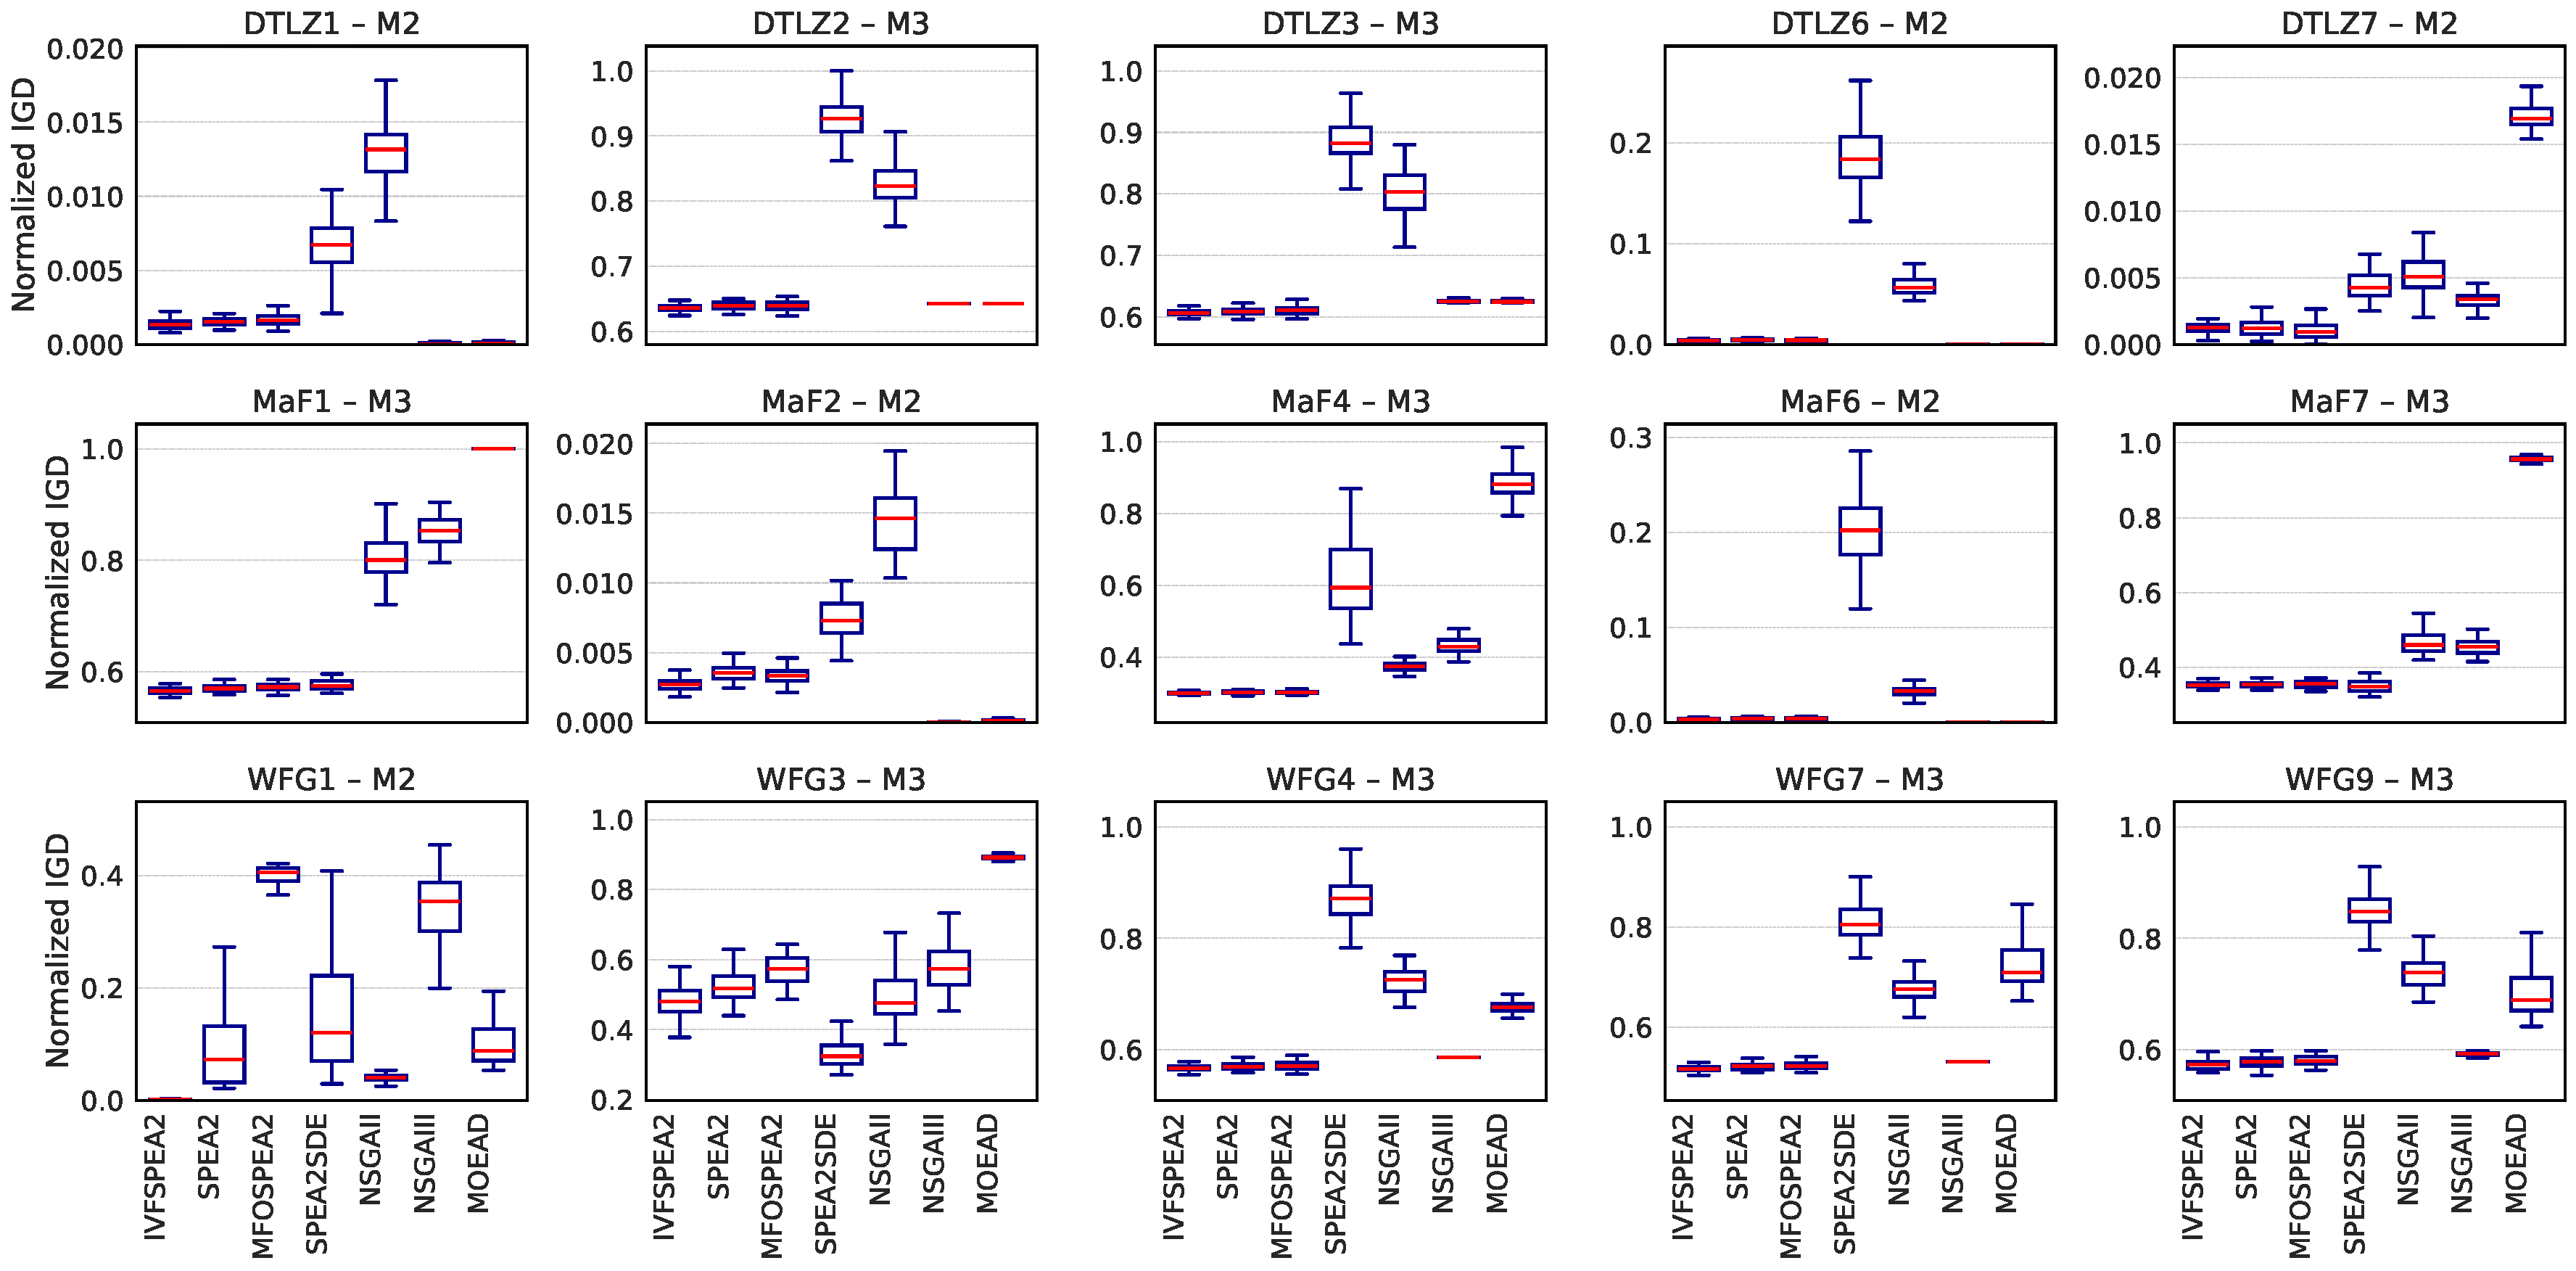
\includegraphics[width=\textwidth]{fig/boxplots_3x5_monocromatico_nome.pdf}
    \caption{Diagramas de caixa dos valores de IGD normalizado para problemas selecionados DTLZ, MaF e WFG, comparando IVF/SPEA2, SPEA2 e outros algoritmos de referência (MFOSPEA2, SPEA2SDE, NSGAII, NSGAIII, MOEAD).}
    \label{fig:boxplots_comparison}
\end{figure}

A análise dos diagramas de caixa na Figura~\ref{fig:boxplots_comparison} revela que o IVF/SPEA2 alcança consistentemente valores medianos de IGD menores na maioria dos problemas de referência, demonstrando qualidade de convergência superior. Particularmente notável é o desempenho do algoritmo em problemas desafiadores como DTLZ3 (M=3), MaF4 (M=3) e problemas WFG, onde o desempenho mediano e variância reduzida indicam tanto melhor qualidade de solução quanto estabilidade algorítmica aprimorada. Os problemas onde o IVF/SPEA2 demonstrou desempenho superior frequentemente compartilham características desafiadoras que testam a capacidade de um algoritmo de equilibrar convergência e diversidade:
\begin{itemize}
    \item \textbf{WFG1, WFG3-5, WFG7-9}: Características incluindo não-separabilidade, decepção, multimodalidade e geometrias complexas de frentes de Pareto~\cite{Huband2006}.
    \item \textbf{MaF1, MaF3, MaF6}: Paisagens complexas e interações objetivas desafiadoras~\cite{Cheng2017}.
    \item \textbf{DTLZ1, DTLZ2, DTLZ5, DTLZ6}: Várias geometrias de frentes de Pareto testando capacidades de convergência.
\end{itemize}

Para um exame mais detalhado do desempenho algorítmico dentro de famílias específicas de problemas de referência, a suíte de teste WFG é analisada separadamente devido à sua reputação por apresentar desafios de otimização diversos. A Figura~\ref{fig:wfg_igd_boxplot} apresenta distribuições de IGD normalizado para todos os nove problemas WFG, segregados por dimensionalidade do espaço objetivo. A comparação foca em três algoritmos chave: IVF/SPEA2, o SPEA2 de referência e MFOSPEA2 como um otimizador multi-objetivo representativo do estado da arte. Esta análise focada permite uma avaliação clara da consistência de desempenho através de problemas com características variadas como viés, não-separabilidade e paisagens enganosas.

\begin{figure}[!htb]
    \centering
    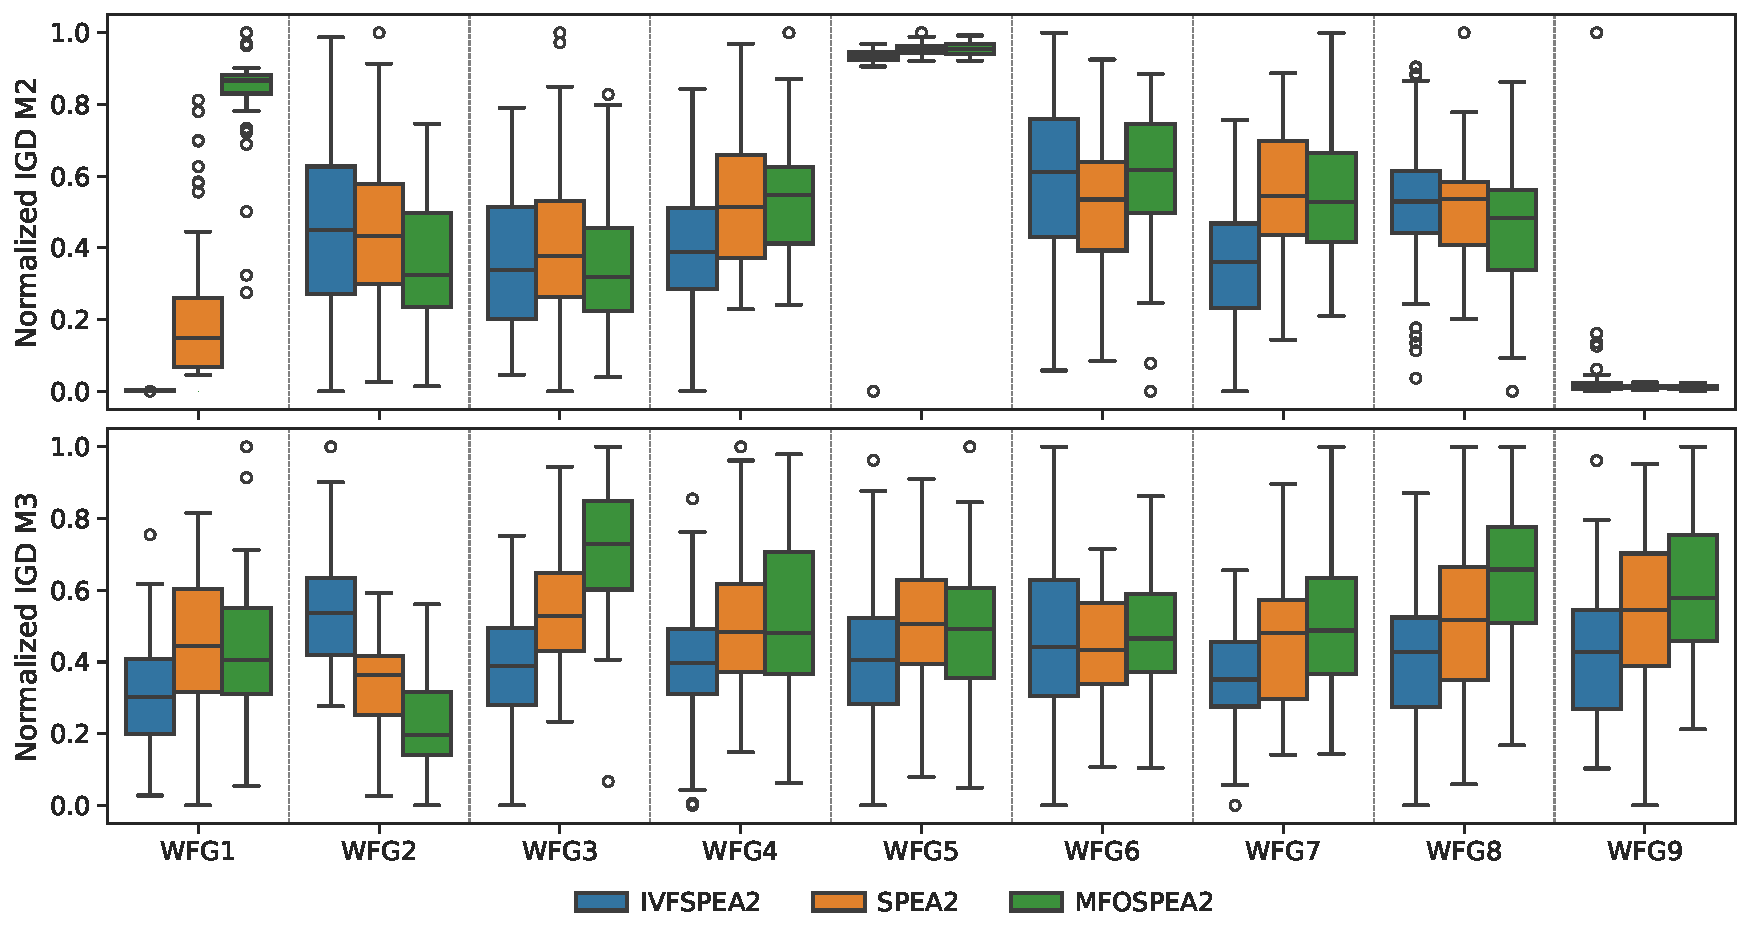
\includegraphics[
    %width=0.95\textwidth,
    height=0.25\textheight]{fig/wfg_igd_boxplot.pdf}
    \caption{Diagramas de caixa do IGD normalizado para problemas WFG (WFG1-WFG9) com M=2 e M=3 objetivos, comparando IVF/SPEA2, SPEA2 e MFOSPEA2. A linha superior exibe resultados para M=2 objetivos, e a linha inferior para M=3 objetivos.}
    \label{fig:wfg_igd_boxplot}
\end{figure}

A análise específica do WFG demonstra o desempenho robusto do IVF/SPEA2 através de toda a suíte, com vantagens particularmente pronunciadas em cenários tri-objetivo (M=3). O algoritmo exibe consistentemente valores medianos de IGD menores e intervalos interquartis reduzidos comparados tanto ao SPEA2 quanto ao MFOSPEA2. Este desempenho superior é especialmente evidente em WFG1, WFG3, WFG4 e WFG7, onde as características desafiadoras dos problemas como viés polinomial e variáveis de decisão não-separáveis tipicamente dificultam otimizadores multi-objetivo convencionais.

Para fornecer uma visão abrangente através de múltiplas famílias de problemas de referência, a Figura~\ref{fig:all_benchmarks_igd_boxplot} apresenta as distribuições de desempenho para as suítes de teste ZDT, DTLZ e MaF. Cada subgráfico representa uma família distinta de problemas de referência, com separação clara entre instâncias de problemas bi-objetivo (M=2) e tri-objetivo (M=3). Os três algoritmos comparados representam paradigmas algorítmicos diferentes: IVF/SPEA2 (abordagem proposta), SPEA2 (método clássico baseado em Pareto) e MFOSPEA2 (variante aprimorada do SPEA2 com gestão melhorada de diversidade). Esta estrutura comparativa permite a avaliação da robustez algorítmica através de diferentes paisagens de problemas e dimensionalidades do espaço objetivo.

\begin{figure}[!htb]
    \centering
    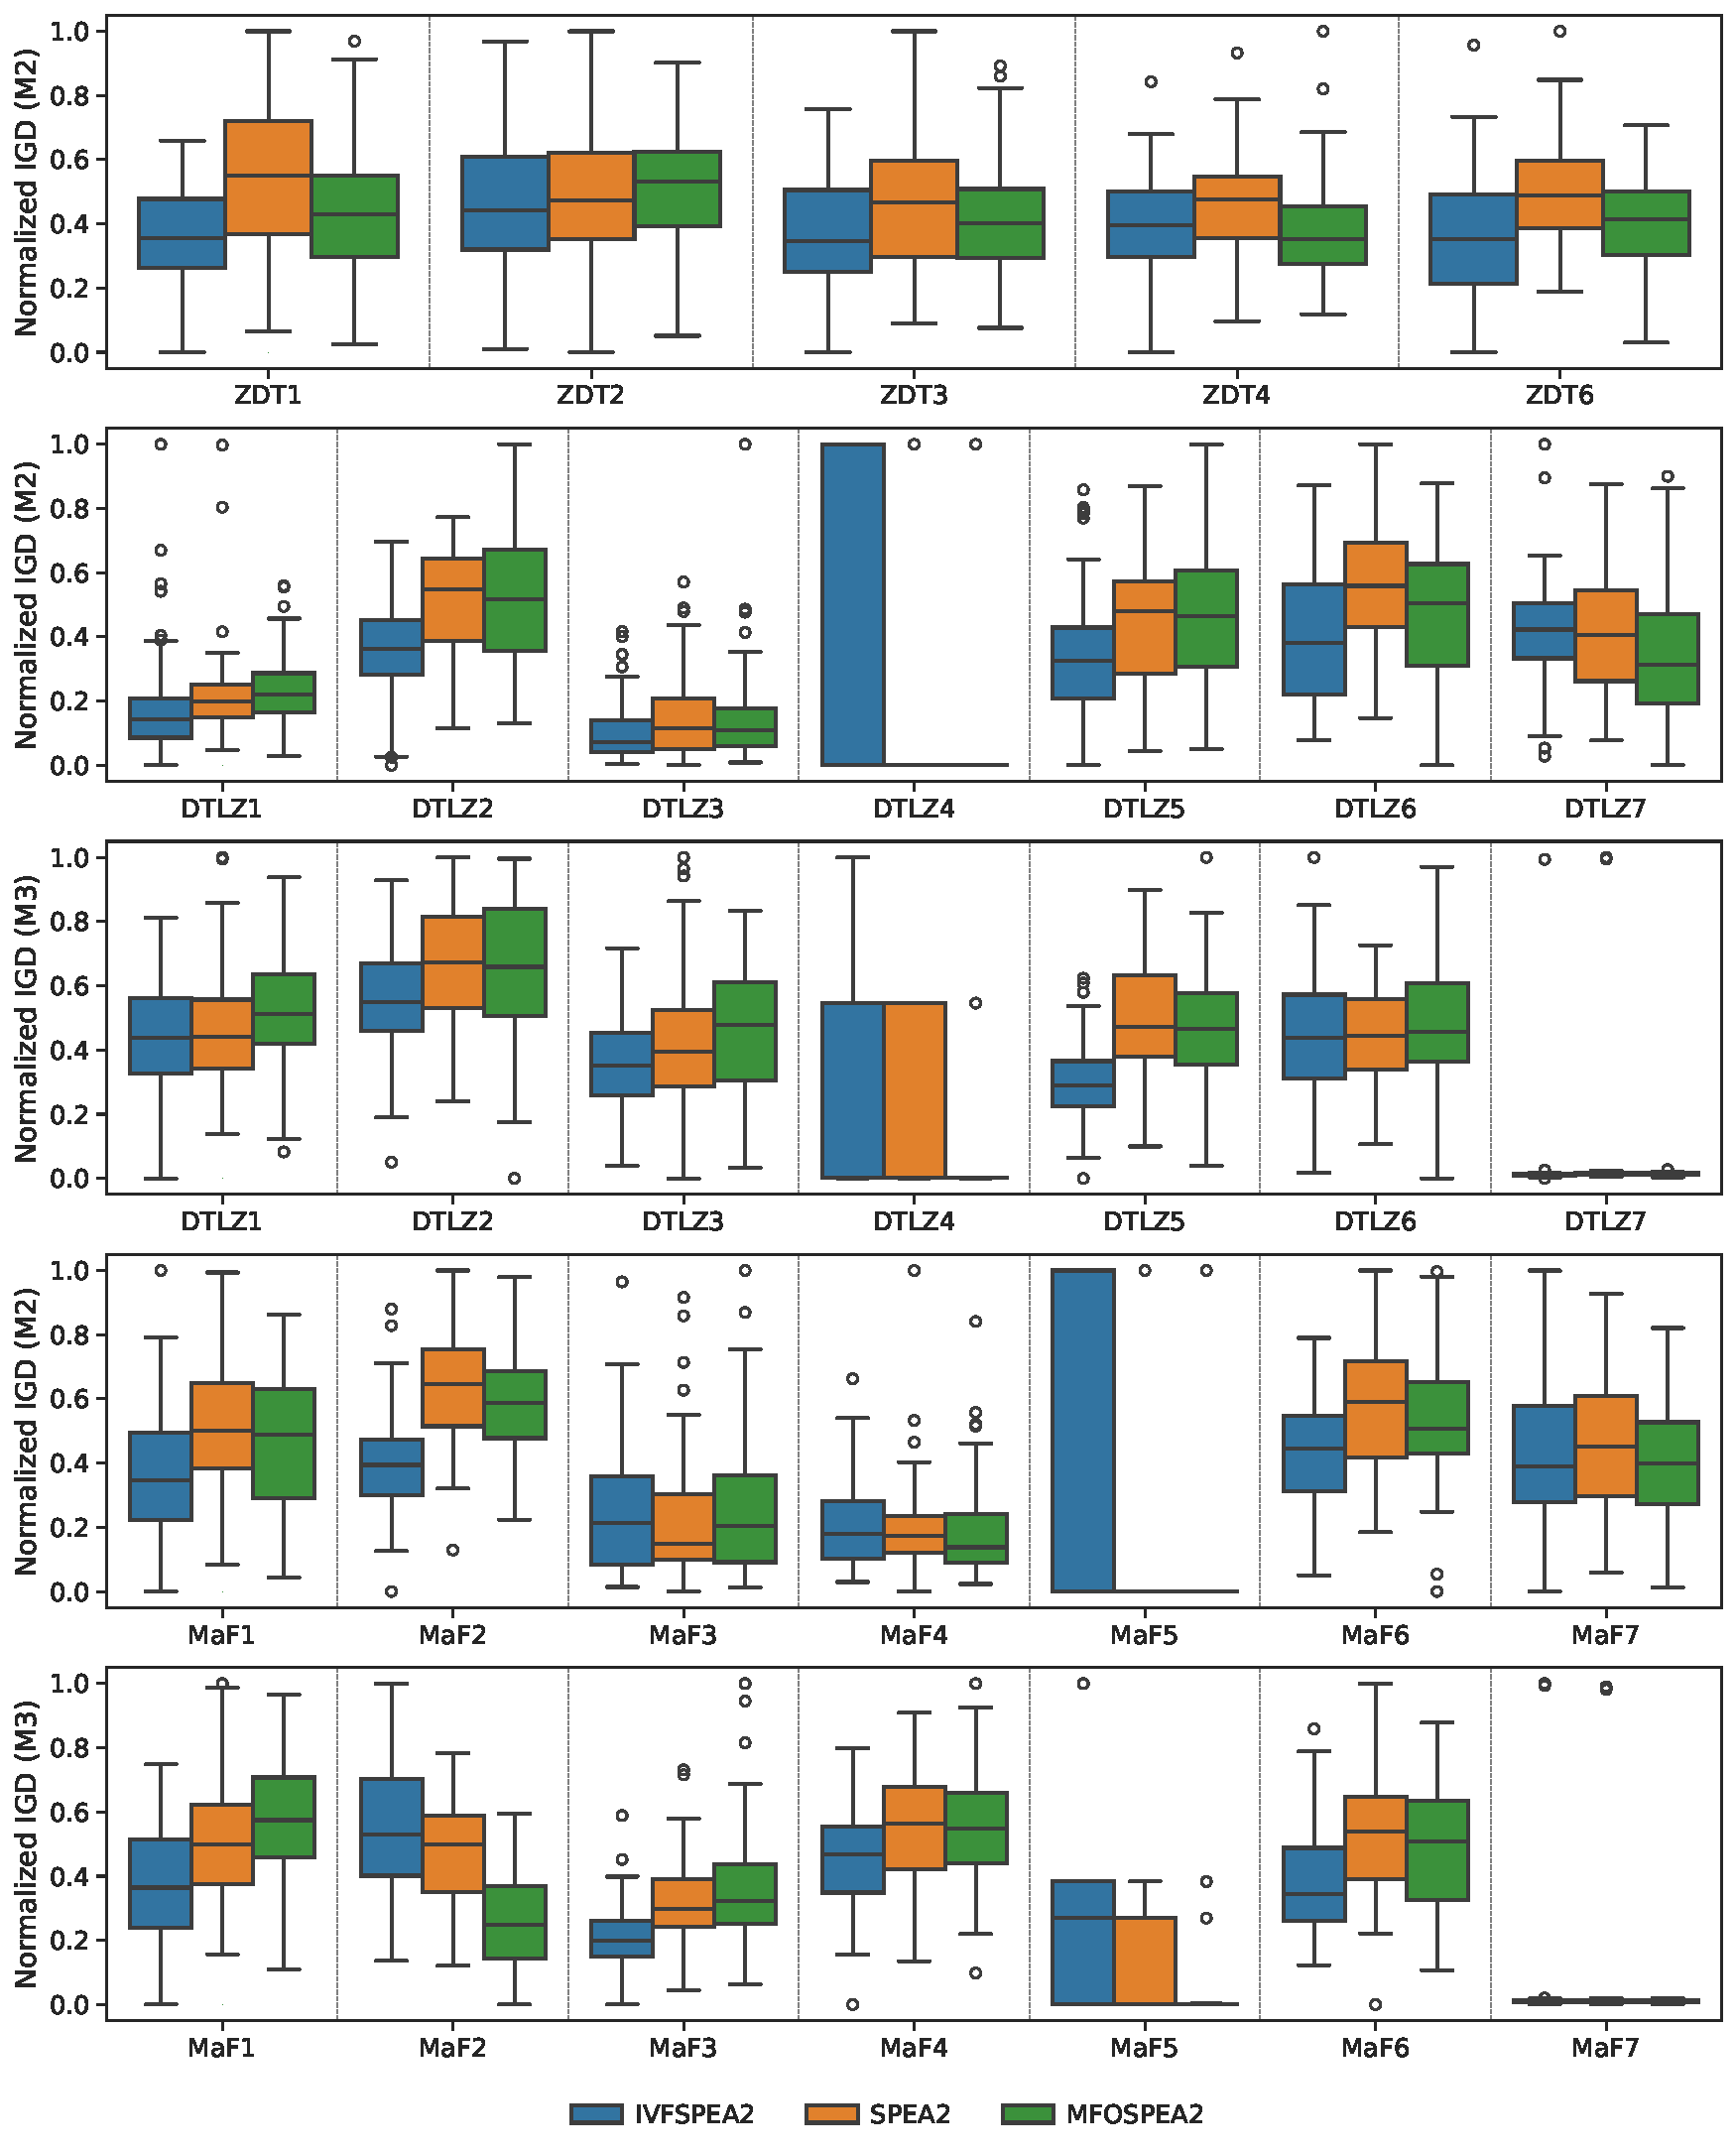
\includegraphics[
    %width=0.95\textwidth,
    height=0.6\textheight]{fig/all_benchmarks_igd_boxplot.pdf}
    \caption{Diagramas de caixa do IGD normalizado para problemas ZDT, DTLZ e MaF (ZDT1-ZDT6, DTLZ1-DTLZ7 e MaF1 - MaF7) com M=2 e M=3 objetivos, comparando IVF/SPEA2, SPEA2 e MFOSPEA2. A linha superior exibe resultados para M=2 objetivos, e a linha inferior para M=3 objetivos para cada problema de referência.}
    \label{fig:all_benchmarks_igd_boxplot}
\end{figure}

A análise abrangente dos problemas de referência revela que o IVF/SPEA2 mantém vantagens consistentes de desempenho através de características diversas de problemas. Na suíte ZDT, o algoritmo demonstra desempenho superior em problemas com frentes de Pareto descontínuas (ZDT3) e paisagens multimodais (ZDT4, ZDT6). Para a família DTLZ, melhorias significativas são observadas particularmente em problemas com frentes de Pareto lineares (DTLZ1, DTLZ2) e geometrias degeneradas (DTLZ5, DTLZ6). Os resultados da suíte MaF confirmam ainda mais a eficácia do algoritmo em problemas multi-objetivo de grande escala e complexos, com ganhos notáveis de desempenho em MaF1, MaF2 e MaF6.

Finalmente, para avaliar a significância prática dessas diferenças de desempenho além de simples comparações de métricas, uma análise estatística rigorosa usando o teste de tamanho de efeito Vargha-Delaney A12 é apresentada. A Figura~\ref{fig:vargha_delaney_comparison_algorithms} exibe os resultados da análise de tamanho de efeito, onde cada célula representa a probabilidade de que o IVF/SPEA2 superará o algoritmo comparado em um dado problema. A análise abrange todos os problemas de referência segregados por dimensionalidade do espaço objetivo, com seis algoritmos competidores: MFOSPEA2, MOEA/D, NSGA-II, NSGA-III, SPEA2 e SPEA2+SDE. A visualização emprega um esquema de codificação por cores para indicar tanto a direção da diferença de desempenho (melhor, igual, pior) quanto a magnitude do tamanho de efeito de acordo com limites estatísticos estabelecidos (negligível, pequeno, médio, grande).

\begin{figure}[!htb]
    \centering
    % Figura para M=2 objetivos (linha superior)
    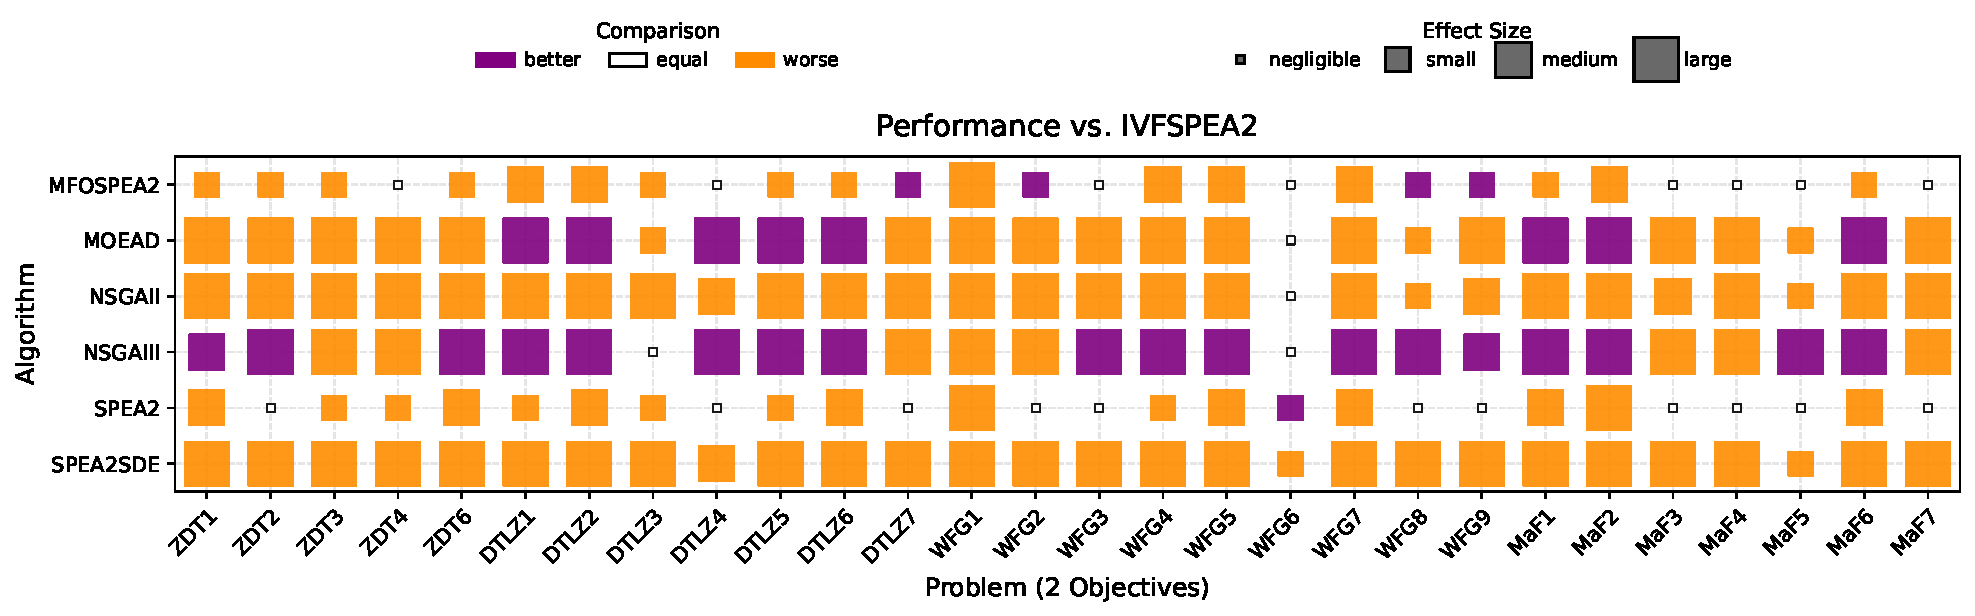
\includegraphics[width=1.0\textwidth]{fig/plot_ZDT_DTLZ_WFG_MaF_M2_Objectives_vs_IVFSPEA2.pdf}
    
    % Espaçamento vertical entre as figuras
    \vspace{0.1cm} 
    
    % Figura para M=3 objetivos (linha inferior)
    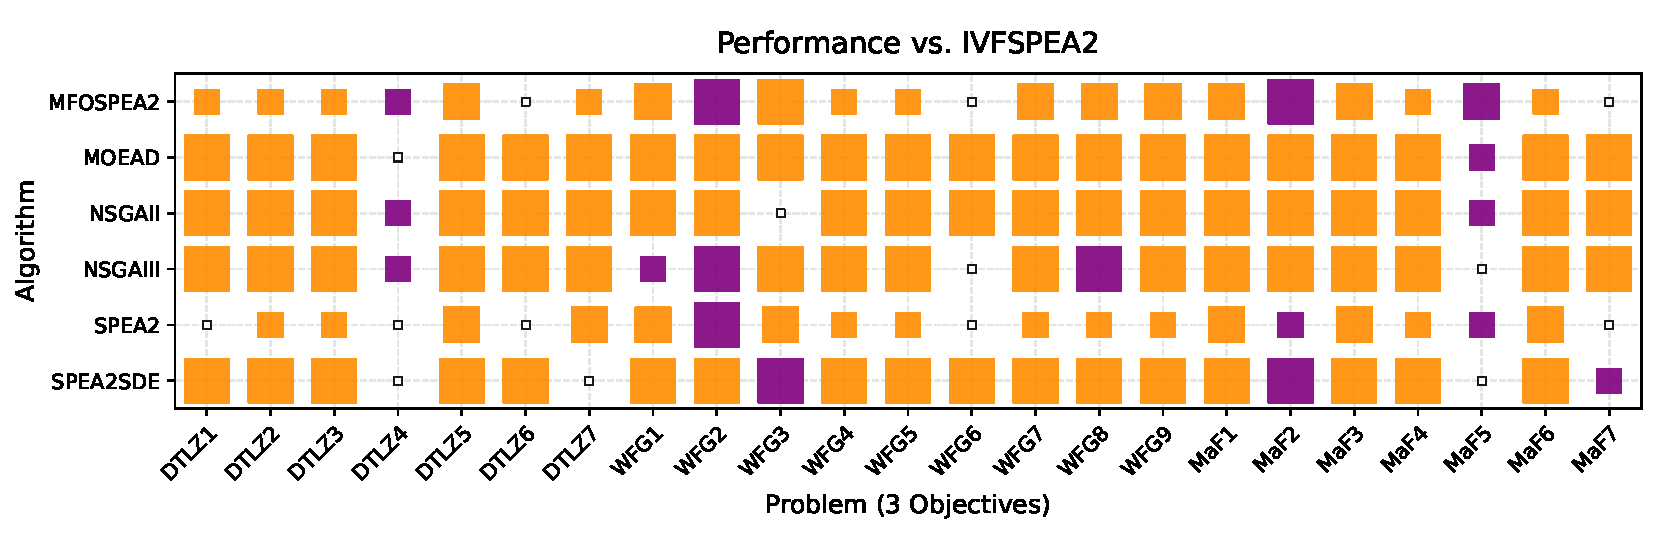
\includegraphics[width=0.85\textwidth]{fig/plot_DTLZ_WFG_MaF_M3_Objectives_vs_IVFSPEA2-b.pdf}
    
    \caption{Análise comparativa de desempenho usando teste de tamanho de efeito Vargha-Delaney para algoritmos de otimização multi-objetivo em problemas de teste de referência. O painel superior mostra resultados para problemas bi-objetivo (M=2): ZDT1-ZDT4, ZDT6, DTLZ1-DTLZ7, WFG1-WFG9 e MaF1-MaF7. O painel inferior apresenta resultados para problemas tri-objetivo (M=3): DTLZ1-DTLZ7, WFG1-WFG9 e MaF1-MaF7. Todos os algoritmos (MFOSPEA2, MOEA/D, NSGA-II, NSGA-III, SPEA2 e SPEA2+SDE) são comparados contra o algoritmo de referência IVF/SPEA2. A codificação por cores indica comparação de desempenho (melhor, igual, pior) e magnitude do tamanho de efeito (negligível, pequeno, médio, grande) de acordo com a estatística A12 de Vargha-Delaney.}
    \label{fig:vargha_delaney_comparison_algorithms}
\end{figure}

A análise de tamanho de efeito fornece evidência do desempenho superior do IVF/SPEA2 com significância estatística. Para problemas bi-objetivo (M=2), o IVF/SPEA2 demonstra vantagens substanciais contra a maioria dos competidores, com tamanhos de efeito predominantemente variando de pequeno a grande através da maioria dos problemas de referência. A dominância de desempenho torna-se ainda mais pronunciada para problemas tri-objetivo (M=3), onde o IVF/SPEA2 exibe superioridade consistente e estatisticamente significativa através dos problemas de referência DTLZ, WFG e MaF contra todos os algoritmos avaliados. Esta análise estatística abrangente reforça que a integração do mecanismo IVF fornece não apenas vantagens mensuráveis mas também praticamente significativas de desempenho através de paisagens diversas de otimização multi-objetivo, estabelecendo a abordagem proposta como um aprimoramento robusto e eficaz para a estrutura SPEA2.